In all experiments, the reward is generated according to:
\eq{
Y_t \sim \begin{cases}
\bernoulli(.5+\epsilon) & \text{if } X_1 = 1 \\
\bernoulli(\frac{.5-(.5+\epsilon)q_1}{1-q_1}) & \text{otherwise}\,.
\end{cases}
}

With $\epsilon \in (0,.5)$. This ensures that 
\eq {
\P{Y|do(X_i = j)} = \begin{cases}
.5+\epsilon & \text{if } (i,j)=(1,1) \\
\frac{.5-(.5+\epsilon)q_1}{1-q_1} & \text{if } (i,j) = (1,0) \\
.5 & \text{otherwise}
\end{cases}
}

This allows us to rapidly simulate rewards and conditional rewards for large numbers of variables and to change the value of $\boldsymbol{q}$ with minimal impact on the reward function \footnote{$\boldsymbol{q}$ only effects the reward of a single, non-optimal arm, which becomes insignificant with large numbers of variables.}. 

\begin{figure}
\caption{Final regret versus number of variables $N$ for UCB with $\alpha = 2$, Causal-Explore-Exploit with $m=2$ and with $m=N$ and horizon $T = 10,000$ . Error bars show standard deviation over 100 simulations. The regret for UCB grows linearly with the number of variables, whist for Causal-Explore-Exploit with fixed $m$, the growth is sub-logarthmic.  }
\label{fig:known_q_r_vs_N}
\centering
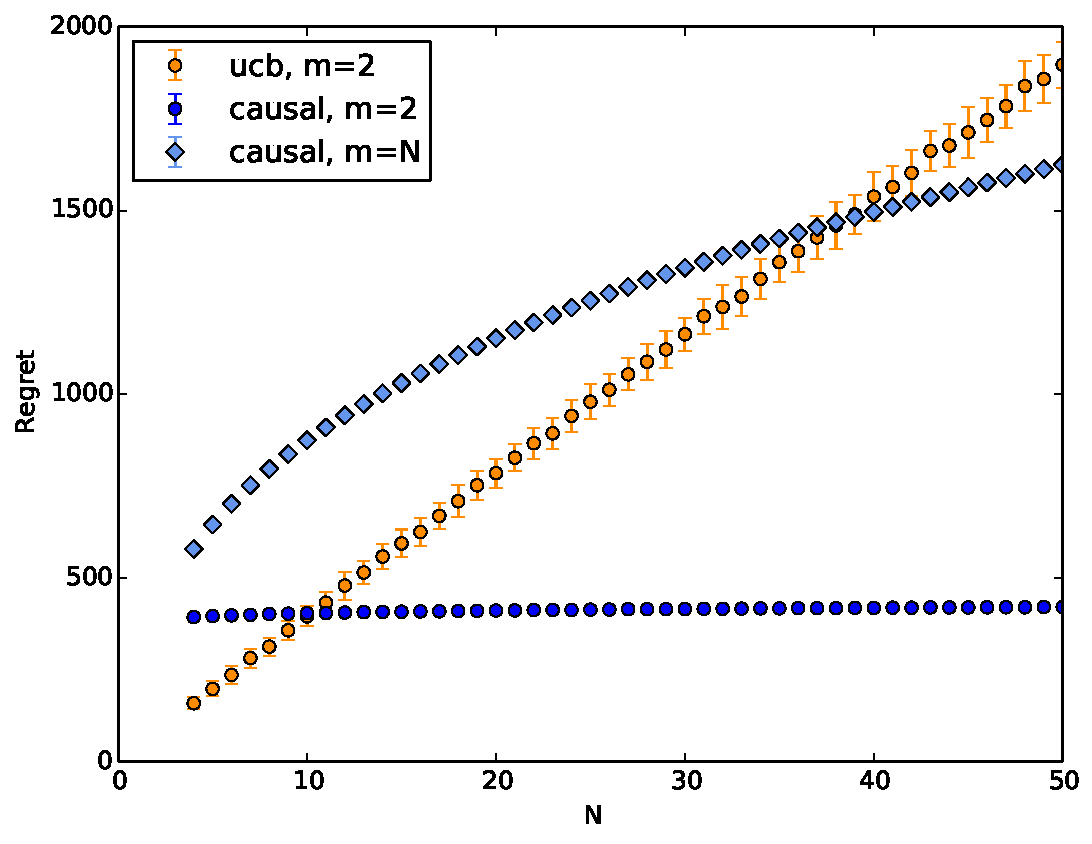
\includegraphics[width=.5\textwidth]{exp_regret_vs_N_T10000_sims100_20151229_113550.pdf}
\end{figure}

\begin{figure}
\caption{Cumulative regret over time for $N = 17$ for UCB with $\alpha=2$, Causal-Explore-Exploit with $m=2$ and Causal-Explore-Exploit with $m=N$. Shaded region shows standard deviation over 100 simulations. The Causal-Explore-Exploit algorithm incurs linear regret during the exploration phase, after which it selects the optimal arm with high probability. For $m=2$, we have $K \sim m^{2/3}T^{1/3}$ and see that we are in the regime in which Causal-Explore-Exploit outperforms UCB.}
\label{fig:known_q_r_vs_t}
\centering
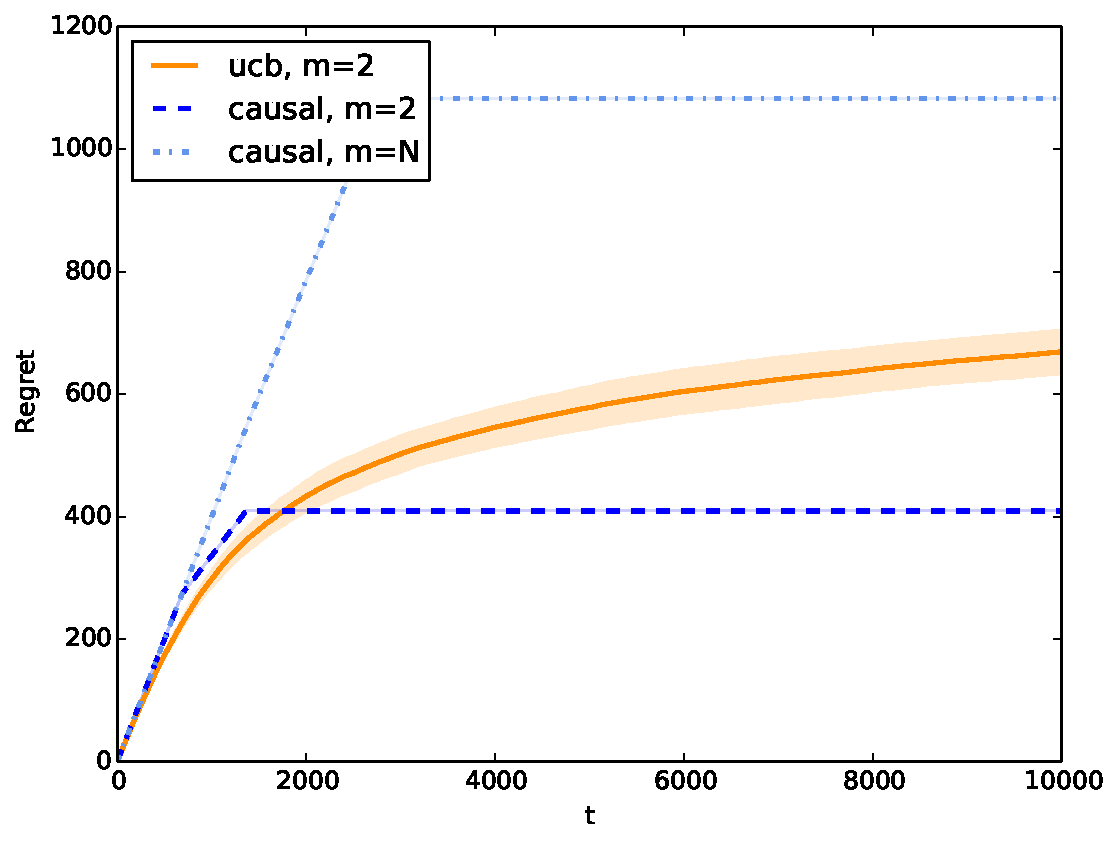
\includegraphics[width=.5\textwidth]{exp_regret_vs_t_T10000_N17_sims100_20151229_120647.pdf}
\end{figure}

\begin{figure}
\caption{Simple regret vs horizon, $T$, for $N = 30$ for UCB with $\alpha=2$, Causal-Best-Arm-Identification with $m=2$ and Causal-Best-Arm-Identification with $m=N$. Error bars show estimated 95\% confidence interval from 1000 simulations.}
\label{fig:simple_vs_T}
\centering
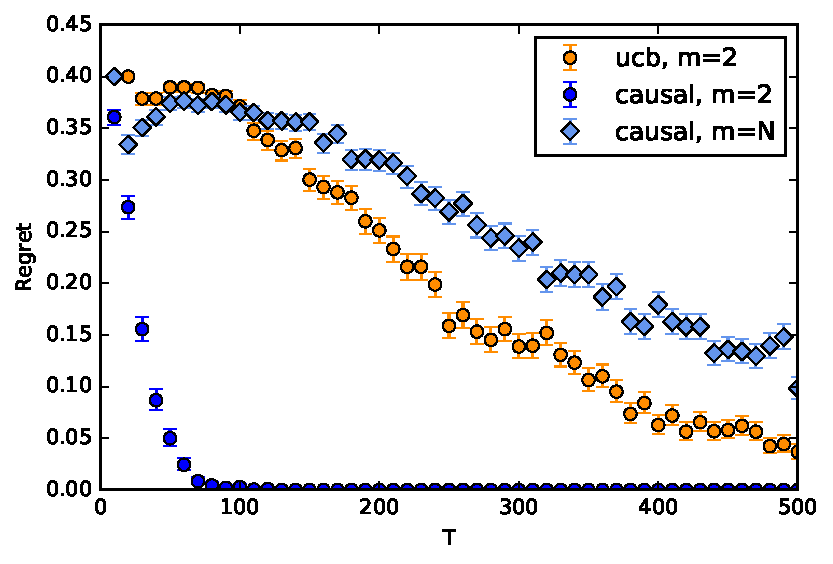
\includegraphics[width=.5\textwidth]{exp_simpleregret_vs_T_N30_sims1000_20160113_010512.pdf}
\end{figure}

\begin{figure}
\caption{Simple regret vs number of variables, $N$, for $T=500$, for UCB with $\alpha=2$, Causal-Best-Arm-Identification with $m=2$ and Causal-Best-Arm-Identification with $m=N$. Error bars show estimated 95\% confidence interval from 1000 simulations.}
\label{fig:simple_vs_N}
\centering
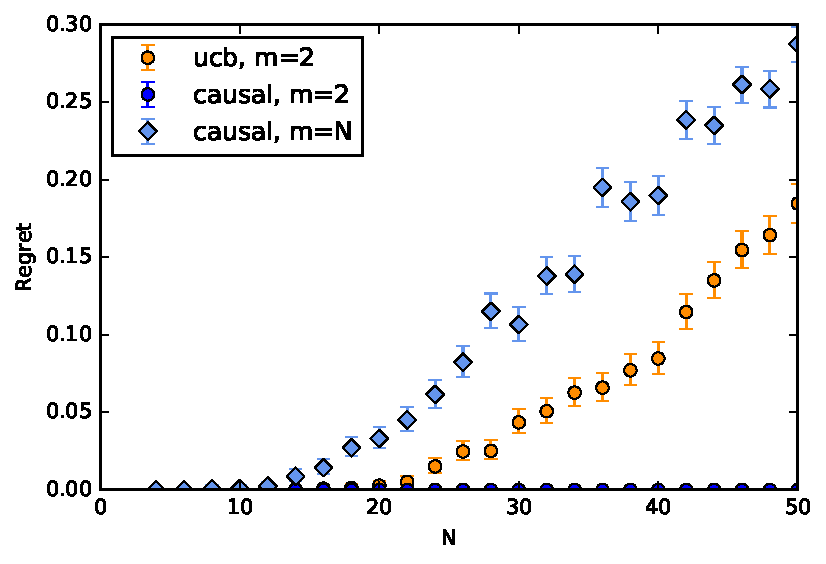
\includegraphics[width=.5\textwidth]{exp_simpleregret_vs_N_T500_sims1000_20160113_010511.pdf}
\end{figure}

